\chapter{Literature Review and Methodology}
\label{chap:review}

If the reader asks a common person in the street what "electronics" means they will receive a variety of responses centred on computers, smartphones, television sets, and other everyday appliances. On the other hand, if the same interviewee demographic was asked about "photonics", some might mention \acl{led}s (\acs{led}s) and lasers, others might cite Star Trek or other science-fiction work. The term photonics has not found widespread understanding outside the semiconductor industry, despite these two technologies often being separated by around a decade and a half in the research and development stages. 

The basic building block of modern electronics, the transistor, was invented in 1947 \cite{Bardeen1948, Bardeen1950}. Pointing to a direct equivalent in the history of photonics is not straightforward; however, the first solid-state light-emitting device was described just \num{15} years later in 1962 \cite{Biard1966} and consisted of a \acf{gaas} \acs{led} emitting in the infrared. Interest in solid-state lasing grew immediately after this discovery \cite{Hall1962, Hall1963} affirming the role of III-V semiconductors as solid-state light emitters. The next year, in 1963, Wanlass invented \acf{cmos} technology \cite{Wanlass1967} cementing integrated planar electronics as the main computational platform of the second half of the century. It took four years after this seminal invention for the idea of a \acf{pic} to follow \cite{Miller1969}.

Therefore, while integrated electronics was entering its exponential phase, exemplified by Moore's law \cite{Moore1965}, formulated in the mid-1960s, the building blocks of photonics were just being discovered or still in a conceptual phase. This led to a difference in investment that, in turn, shaped the technological landscape of humanity. While commercial electron-based technologies were progressing through small-, medium- and large-scale integration, up until very large-scale, photon-based technology was mostly commercialised as bulk devices for, until the discovery of the blue \acs{led} in the 1990s \cite{Nakamura1994}, highly specialised lighting applications, and solid-state lasers. However, the 1990s saw a new revolution: the introduction, and rapid diffusion, of the Internet. This new technology exposed the limitation of the electron as an information-carrying particle: impedance losses and inductive currents can be sidestepped by choosing to transmit information with pulses of light because induction is an issue specific to electron-based technology. Simultaneously, the fibre optic cable can support a larger data stream than copper wires. The switch from metallic cables to optical supports was quickly implemented in the long-range communication infrastructure, going hand in hand with the employment of bulk emitters and absorbers at the two ends of the cable. This change also stimulated interest in the use of this technology in integrated interconnects, which has been growing since the late 1980s \cite{Miller1989}.

In integrated interconnects the use of photons bypasses some important problems affecting electrical lines, such as the "aspect ratio limit" that binds the maximum amount of bits per second to the shape of the interconnect \cite{Miller1997}, the dependence of clock timing on temperature, cross-talk between neighbouring interconnects, and the transition between high impedance electronic components and low impedance electronic interconnects, while providing voltage isolation and potential for free space interconnects \cite{Miller1997_reasons}. Most of these problems also have electrical solutions. Still, these solutions in turn increase the energy requirements and therefore the energy loss that occurs on the circuit board, and there is a limit to how much heat can be cost-effectively extracted from each singular chip; therefore, photonics becomes attractive from both an energy- and a cost-efficiency point of view \cite{Miller2009}, provided that the integration method allows such an efficiency. 

Indeed, integration is the key step in enabling photonics. The initial photonic circuits of the late 1980s and 1990s were realised directly on \acf{inp} wafers from \num{2} inches to \num{4} inches in diameter. Despite the small size, these are expensive supports compared to the much larger \qty{150}{\milli\metre} and \qty{200}{\milli\metre} \acl{si} supports their contemporary. This technology managed to demonstrate very large scale integration by the mid-2010s, after which it was surpassed by both \acl{si} and III-V on \acl{si} photonic integrated circuits \cite{Shekhar2024, Margalit2021}.

An important objective is to perfect the integration of efficient III-V components on the cheap \acl{si} substrate. The main issue that needs to be addressed in the integration of III-V semiconductors on \acl{si} is the mismatch in the lattice parameter between these two materials, which causes a wide variety of defects in monolithic integration \cite{Kunert2018}. 

\section{Properties of III-V materials}

\begin{figure}
    \centering
    \subcaptionbox{
        \hkl{0 0 1} facet.
        \label{subfig:GaAs_100}
    }{
        \tikzsetnextfilename{GaAs_100}
        \begin{tikzpicture}
            \node[inner sep=0pt] (image) at (0, 0) {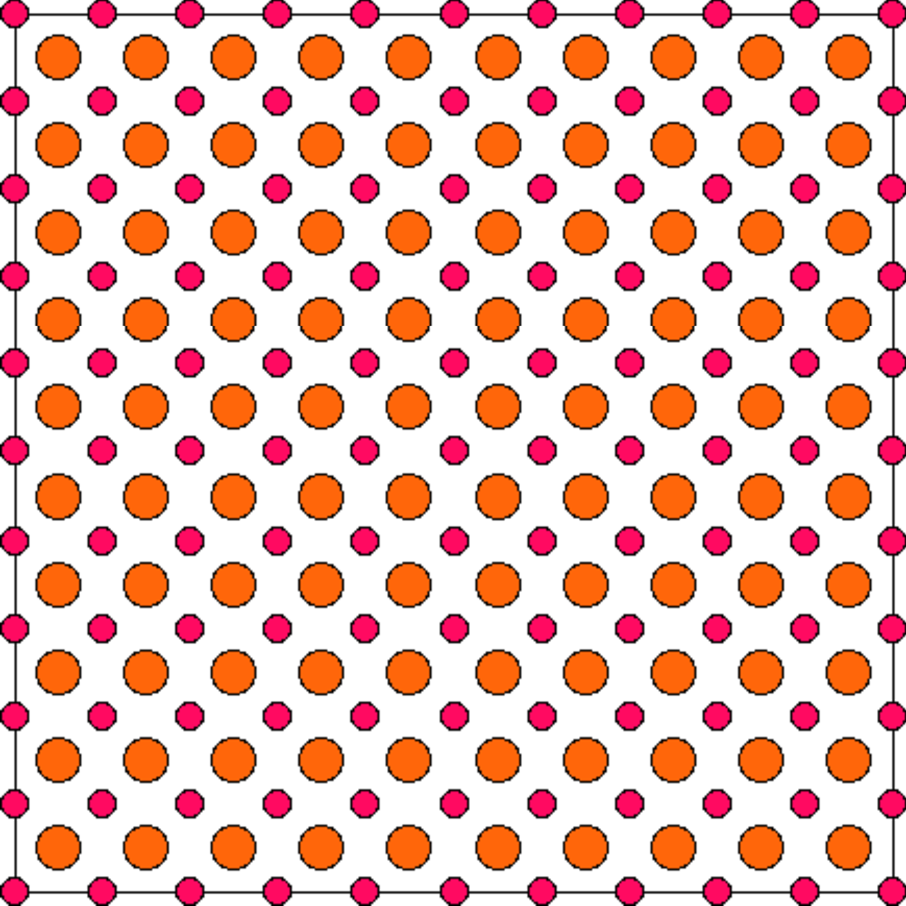
\includegraphics[width=0.30\textwidth]{2_Literature_Review/Fig/GaAs_100.pdf}};
            \draw [fill = black] (0.15, 0.15) rectangle (-0.15, -0.15);
            \draw [white] (0.1, 0.1) -- (-0.1, -0.1);
            \draw [white] (-0.1, 0.1) -- (0.1, -0.1);
        \end{tikzpicture}
    }
    \subcaptionbox{
        \hkl{1 1 0} facet.
        \label{subfig:GaAs_110}
    }{
        \tikzsetnextfilename{GaAs_110}
        \begin{tikzpicture}
            \node[inner sep=0pt] (image) at (0, 0) {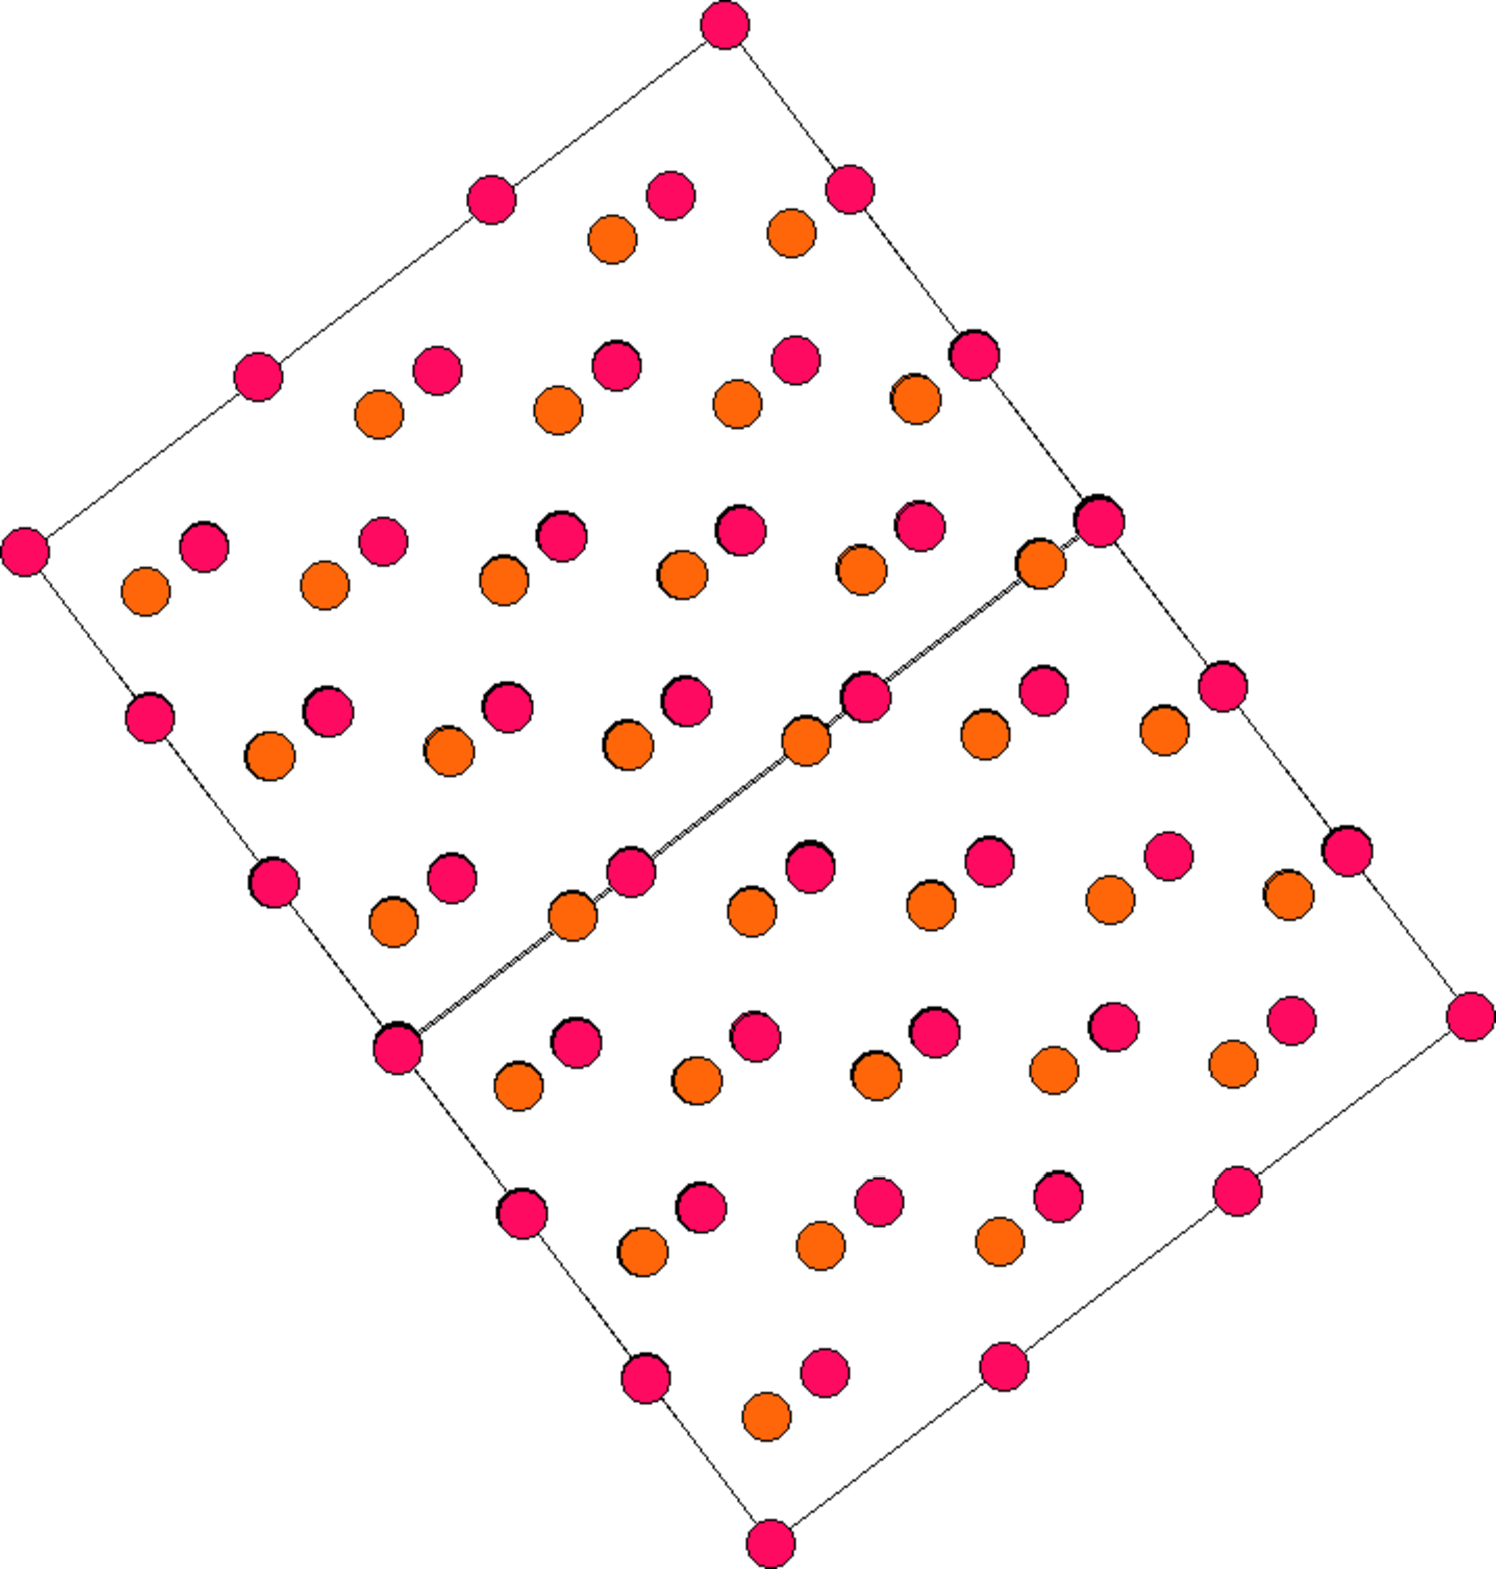
\includegraphics[width=0.30\textwidth]{2_Literature_Review/Fig/GaAs_110.pdf}};
            \begin{scope}[yshift=-0.01]
                \draw (0, 0) -- ++ (37:2);
                \draw (0, 0) -- ++ (37:-2);
                \draw (34:1.9) -- ++ (37:-0.3) -- ++ (-53:0.1) -- cycle;
                \draw (40:1.9) -- ++ (37:-0.3) -- ++ (127:0.1) -- cycle;
            \end{scope}
        \end{tikzpicture}
    }
    \subcaptionbox{
        \hkl{1 1 1}\(_B\) facet.
        \label{subfig:GaAs_111}
    }{
        \tikzsetnextfilename{GaAs_111}
        \begin{tikzpicture}
            \node[inner sep=0pt] (image) at (0, 0) {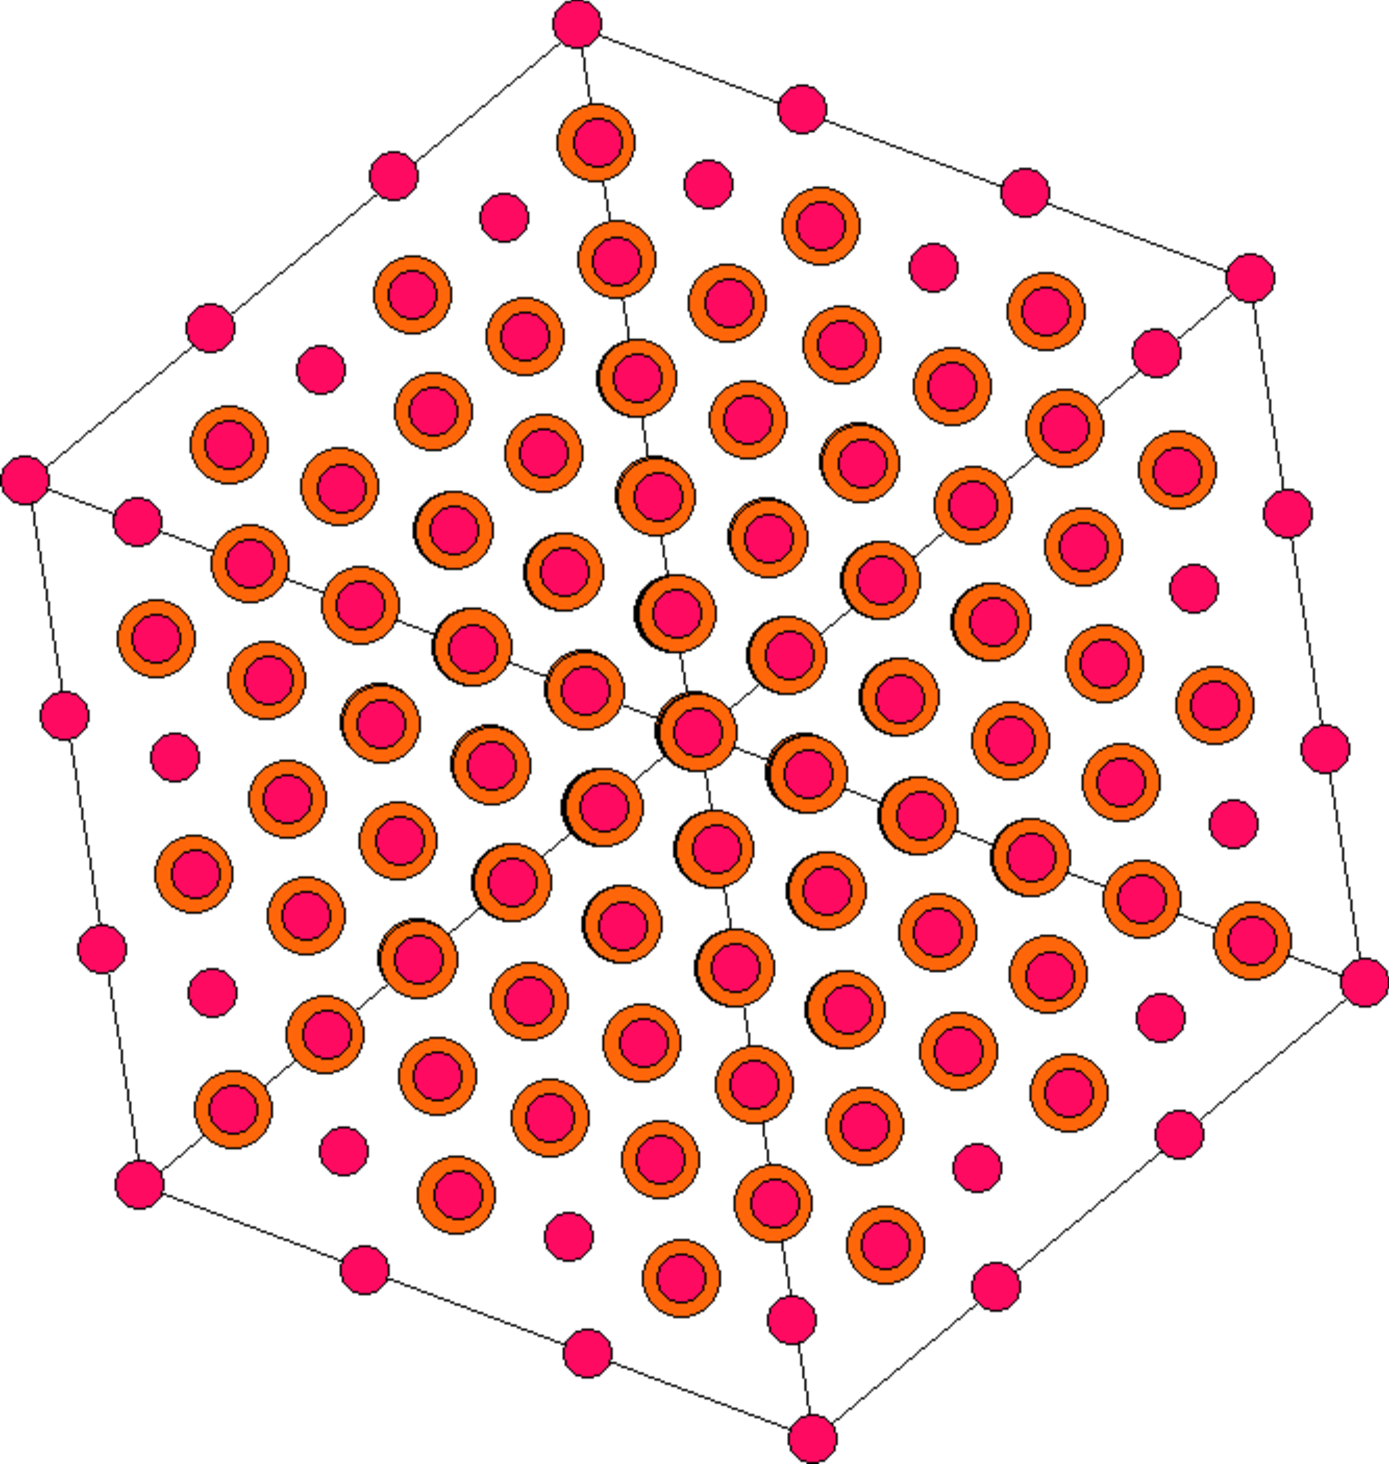
\includegraphics[width=0.30\textwidth]{2_Literature_Review/Fig/GaAs_111.pdf}};
            \draw [fill = black] (0.17, 0) -- ++ (-150:0.3) -- ++ (90:0.3) -- cycle;
            \draw [white] (0, 0) -- ++ (-120:0.1);
            \draw [white] (0, 0) -- ++ (0:0.1);
            \draw [white] (0, 0) -- ++ (120:0.1);
        \end{tikzpicture}
    }
    \caption[Low-index facets in the F\(\bar{4}\)3m \acs{gaas} crystal.]{Simulation of the low-index facets in the F\(\bar{4}\)3m \acs{gaas} crystal with the basic symmetry elements highlighted. \Acl{ga} is represented in orange and \acs{as} in pink; atomic radii are not to scale. \subref{subfig:GaAs_100} shows the 2D projection of the lattice along the \hkl{0 0 1} direction, which coincides with the four-fold axis. \subref{subfig:GaAs_110} shows the 2D projection along the \hkl{1 1 0} direction, contained in the mirror plane. \subref{subfig:GaAs_111} shows the 2D projection along the \hkl{1 1 1} direction, coinciding with the three-fold axis.}
    \label{fig:ZB_low_index_facets}
\end{figure}

III-V semiconductors are compound semiconductors formed by the stoichiometric combination of elements from group III and group V of the periodic table. In their simplest form, they are binary, consisting of one element from group III and one from group V, with some examples being \acs{inp} and \acs{gaas}. Ternary and quaternary III-V materials such as \ce{In1_-_xGa_xAs} or \ce{In1_-_xGa_xAs1_-_yP_y} contain three or four different elements, respectively. 

Crystallographically, III-V materials are available at room temperature in crystals with the symmetries of space group number \num{216} (F\(\bar{4}\)3m, or zincblende-like) or \num{186} (P6\(_3\)mc, or wurtzite-like) and are easily affected by polytypism when grown. Space group \num{216} is that of a cubic face-centred crystal, while space group \num{186} describes a hexagonal crystal. These two structures are closely related, as the addition of a two-fold axis alongside the three-fold axis of space group \num{216} results in a phase change to space group \num{186}, transforming the \hkl<1 1 1> direction in the zincblende phase to the \hkl<0 0 0 1> direction in the wurtzite phase. \hkl{1 1 1} facets can also be described according to which half of the AB stoichiometry of the III-V material is exposed. For example, in Figure~\ref{subfig:GaAs_111} the top layer is entirely composed of V atoms. This facet is called a \hkl{1 1 1}\(_B\) facet, while a \hkl{1 1 1}\(_A\) facet has III atoms exposed.

Figure~\ref{fig:ZB_low_index_facets} shows the 2D projections of a \acs{gaas} F\(\bar{4}\)3m crystal along the low-index directions. These projections are useful for interpreting atomic-resolution microscopy images of III-V semiconductors. These simulated projections were created using CrystalKit, a dedicated software. They also highlight the main symmetry elements of the zincblende space group. The 2D projection in Figure~\ref{subfig:GaAs_100} shows how a \hkl{0 0 1} facet appears in the microscope. The symmetry element controlling its motif is a four-fold axis perpendicular to the projection plane. Similarly, Figure~\ref{subfig:GaAs_110} shows how a \hkl{1 1 0} facet appears in the microscope and the mirror plane dictating its symmetry. Finally, Figure~\ref{subfig:GaAs_111} shows the lattice projected along the \hkl<1 1 1> direction. The symmetry of this projection is compatible with a three-fold axis coinciding with the \hkl<1 1 1> vector.

\begin{figure}
    \centering
    \subcaptionbox{
        \hkl[0 0 1] corresponding to the z-axis.
        \label{subfig:100_symmetry}
    }{
        \tikzsetnextfilename{100_symmetry}
        \begin{tikzpicture}[isometric]
            \draw [fill=cb1_orange] (0.5, 0.5, 1.5) -- (-0.5, 0.5, 1.5) -- (-0.5, -0.5, 1.5) -- (0.5, -0.5, 1.5) -- cycle;
            % \draw [fill=red] (0.5, 0.5, -1.5) -- (-0.5, 0.5, -1.5) -- (-0.5, -0.5, -1.5) -- (0.5, -0.5, -1.5) -- cycle;
            \draw [fill=cb1_orange] (1.5, 0.5, 0.5) -- (1.5, -0.5, 0.5) -- (1.5, -0.5, -0.5) -- (1.5, 0.5, -0.5) -- cycle;
            % \draw [fill=green] (-1.5, 0.5, 0.5) -- (-1.5, -0.5, 0.5) -- (-1.5, -0.5, -0.5) -- (-1.5, 0.5, -0.5) -- cycle;
            \draw [fill=cb1_orange] (0.5, 1.5, 0.5) -- (-0.5, 1.5, 0.5) -- (-0.5, 1.5, -0.5) -- (0.5, 1.5, -0.5) -- cycle;
            % \draw [fill=blue] (0.5, -1.5, 0.5) -- (-0.5, -1.5, 0.5) -- (-0.5, -1.5, -0.5) -- (0.5, -1.5, -0.5) -- cycle;
            \draw [fill=cb1_light_blue] (1.5, 0.5, 0.5) -- (1.5, -0.5, 0.5)-- (0.5, -0.5, 1.5) -- (0.5, 0.5, 1.5)  -- cycle;
            \draw [fill=cb1_purple] (0.5, 0.5, 1.5)  -- (1.5, 0.5, 0.5) -- (0.5, 1.5, 0.5) -- cycle;
            \draw [fill=cb1_purple] (0.5, -0.5, 1.5)  -- (1.5, -0.5, 0.5) -- (0.5, -1.5, 0.5) -- cycle;
            \draw [fill=cb1_light_blue] (0.5, 0.5, 1.5) -- (-0.5, 0.5, 1.5) -- (-0.5, 1.5, 0.5) -- (0.5, 1.5, 0.5) -- cycle;
            \draw [fill=cb1_light_blue] (0.5, 1.5, -0.5) -- (0.5, 1.5, 0.5) -- (1.5, 0.5, 0.5) -- (1.5, 0.5, -0.5) -- cycle;
            \draw [fill=cb1_purple] (0.5, 0.5, -1.5) -- (0.5, 1.5, -0.5) -- (1.5, 0.5, -0.5) -- cycle;
            \draw [fill=cb1_purple] (-0.5, 0.5, 1.5) -- (-0.5, 1.5, 0.5) -- (-1.5, 0.5, 0.5) -- cycle;
            \draw [-stealth] (0,0,1.5) -- ++ (0,0,1) node [anchor=east] {\hkl[1 0 0]};
            \draw [-stealth] (0,1.5,0) -- ++ (0,1,0) node [anchor=south] {\hkl[0 0 1]};
            \draw [-stealth] (1.5,0,0) -- ++ (1,0,0) node [anchor=west] {\hkl[0 1 0]};
        \end{tikzpicture}
    }
    \subcaptionbox{
        \hkl[1 1 0] corresponding to the z-axis.
        \label{subfig:110_symmetry}
    }{
        \tikzsetnextfilename{110_symmetry}
        \begin{tikzpicture}[isometric]
            \begin{scope}[rotate around x=45]
                \draw [fill=cb1_orange] (0.5, 0.5, 1.5) -- (-0.5, 0.5, 1.5) -- (-0.5, -0.5, 1.5) -- (0.5, -0.5, 1.5) -- cycle;
                \draw [fill=red] (0.5, 0.5, -1.5) -- (-0.5, 0.5, -1.5) -- (-0.5, -0.5, -1.5) -- (0.5, -0.5, -1.5) -- cycle;
                \draw [fill=cb1_orange] (1.5, 0.5, 0.5) -- (1.5, -0.5, 0.5) -- (1.5, -0.5, -0.5) -- (1.5, 0.5, -0.5) -- cycle;
                % \draw [fill=green] (-1.5, 0.5, 0.5) -- (-1.5, -0.5, 0.5) -- (-1.5, -0.5, -0.5) -- (-1.5, 0.5, -0.5) -- cycle;
                \draw [fill=cb1_orange] (0.5, 1.5, 0.5) -- (-0.5, 1.5, 0.5) -- (-0.5, 1.5, -0.5) -- (0.5, 1.5, -0.5) -- cycle;
                % \draw [fill=blue] (0.5, -1.5, 0.5) -- (-0.5, -1.5, 0.5) -- (-0.5, -1.5, -0.5) -- (0.5, -1.5, -0.5) -- cycle;
                \draw [fill=cb1_light_blue] (1.5, 0.5, 0.5) -- (1.5, -0.5, 0.5) -- (0.5, -0.5, 1.5) -- (0.5, 0.5, 1.5)  -- cycle;
                \draw [fill=cb1_purple] (0.5, 0.5, 1.5)  -- (1.5, 0.5, 0.5) -- (0.5, 1.5, 0.5) -- cycle;
                % \draw [fill=cb1_purple] (0.5, -0.5, 1.5)  -- (1.5, -0.5, 0.5) -- (0.5, -1.5, 0.5) -- cycle;
                \draw [fill=cb1_light_blue] (0.5, 0.5, 1.5) -- (-0.5, 0.5, 1.5) -- (-0.5, 1.5, 0.5) -- (0.5, 1.5, 0.5) -- cycle;
                \draw [fill=cb1_light_blue] (0.5, 1.5, -0.5) -- (0.5, 1.5, 0.5) -- (1.5, 0.5, 0.5) -- (1.5, 0.5, -0.5) -- cycle;
                \draw [fill=cb1_purple] (0.5, 0.5, -1.5) -- (0.5, 1.5, -0.5) -- (1.5, 0.5, -0.5) -- cycle;
                \draw [fill=cb1_purple] (-0.5, 0.5, 1.5) -- (-0.5, 1.5, 0.5) -- (-1.5, 0.5, 0.5) -- cycle;
                \draw [fill=cb1_light_blue] (-0.5, 0.5, -1.5) -- (-0.5, 1.5, -0.5) -- (0.5, 1.5, -0.5) -- (0.5, 0.5, -1.5) -- cycle;
                \draw [fill=cb1_light_blue] (1.5, -0.5, -0.5) -- (1.5, 0.5, -0.5) -- (0.5, 0.5, -1.5) -- (0.5, -0.5, -1.5) -- cycle;
                \draw [fill=cb1_light_blue] (-1.5, 0.5, -0.5) -- (-1.5, 0.5, 0.5) -- (-0.5, 1.5, 0.5) -- (-0.5, 1.5, -0.5) -- cycle;
                \draw [fill=cb1_purple] (-0.5, 0.5, -1.5) -- (-1.5, 0.5, -0.5) -- (-0.5, 1.5, -0.5) -- cycle;
                \draw [-stealth] (0,0,-1.5) -- ++ (0,0,-1) node [anchor=south] {\hkl[1 0 0]};
                \draw [-stealth] (0,1.5,0) -- ++ (0,1,0) node [anchor=east] {\hkl[0 1 0]};
                \draw [-stealth] (1.5,0,0) -- ++ (1,0,0) node [anchor=west] {\hkl[0 0 1]};
            \end{scope}
        \end{tikzpicture}
    }
    \caption[Low index facet orientation in the F\(\bar{4}\)3m space group.]{Low index facet orientation in the F\(\bar{4}\)3m space group. The \hkl{0 0 1}, \hkl{1 1 0}, and \hkl{1 1 1} facets are color-coded in orange, light blue, and purple, respectively. The two orientations shown in this Figure are with the vertical z-axis coinciding with the \hkl[0 0 1] and \hkl[1 1 0] directions in \subref{subfig:100_symmetry} and \subref{subfig:110_symmetry}, respectively.}
    \label{fig:facet_relations}
\end{figure}

Although the orientation of the low index facets with respect to each other is difficult to properly convey on a 2D support, Figure~\ref{fig:facet_relations} shows how the three different facets, \hkl{0 0 1} in orange, \hkl{1 1 0} in light blue, and \hkl{1 1 1} in purple, are orientated in a cubic crystal. The shapes of the polygons that make up the figure also give a hint as to what kind of symmetry element is present in each facet. Figure~\ref{subfig:100_symmetry} can also be used to understand the relationship between different planes in the cubic \acl{si} crystal of the \hkl(0 0 1) \acf{soi} device layer used as seed in Chapter~\ref{chap:growth}. Similarly, Figure~\ref{subfig:110_symmetry} illustrates the symmetry of the \hkl(1 1 0) \acs{soi} device layer used in Chapters~\ref{chap:properties} and \ref{chap:yield_analysis}.

\begin{figure}
    \centering
    \tikzsetnextfilename{GaAs_rtp}
    \begin{tikzpicture}
        \node[inner sep=0pt] (image) at (0, 0) {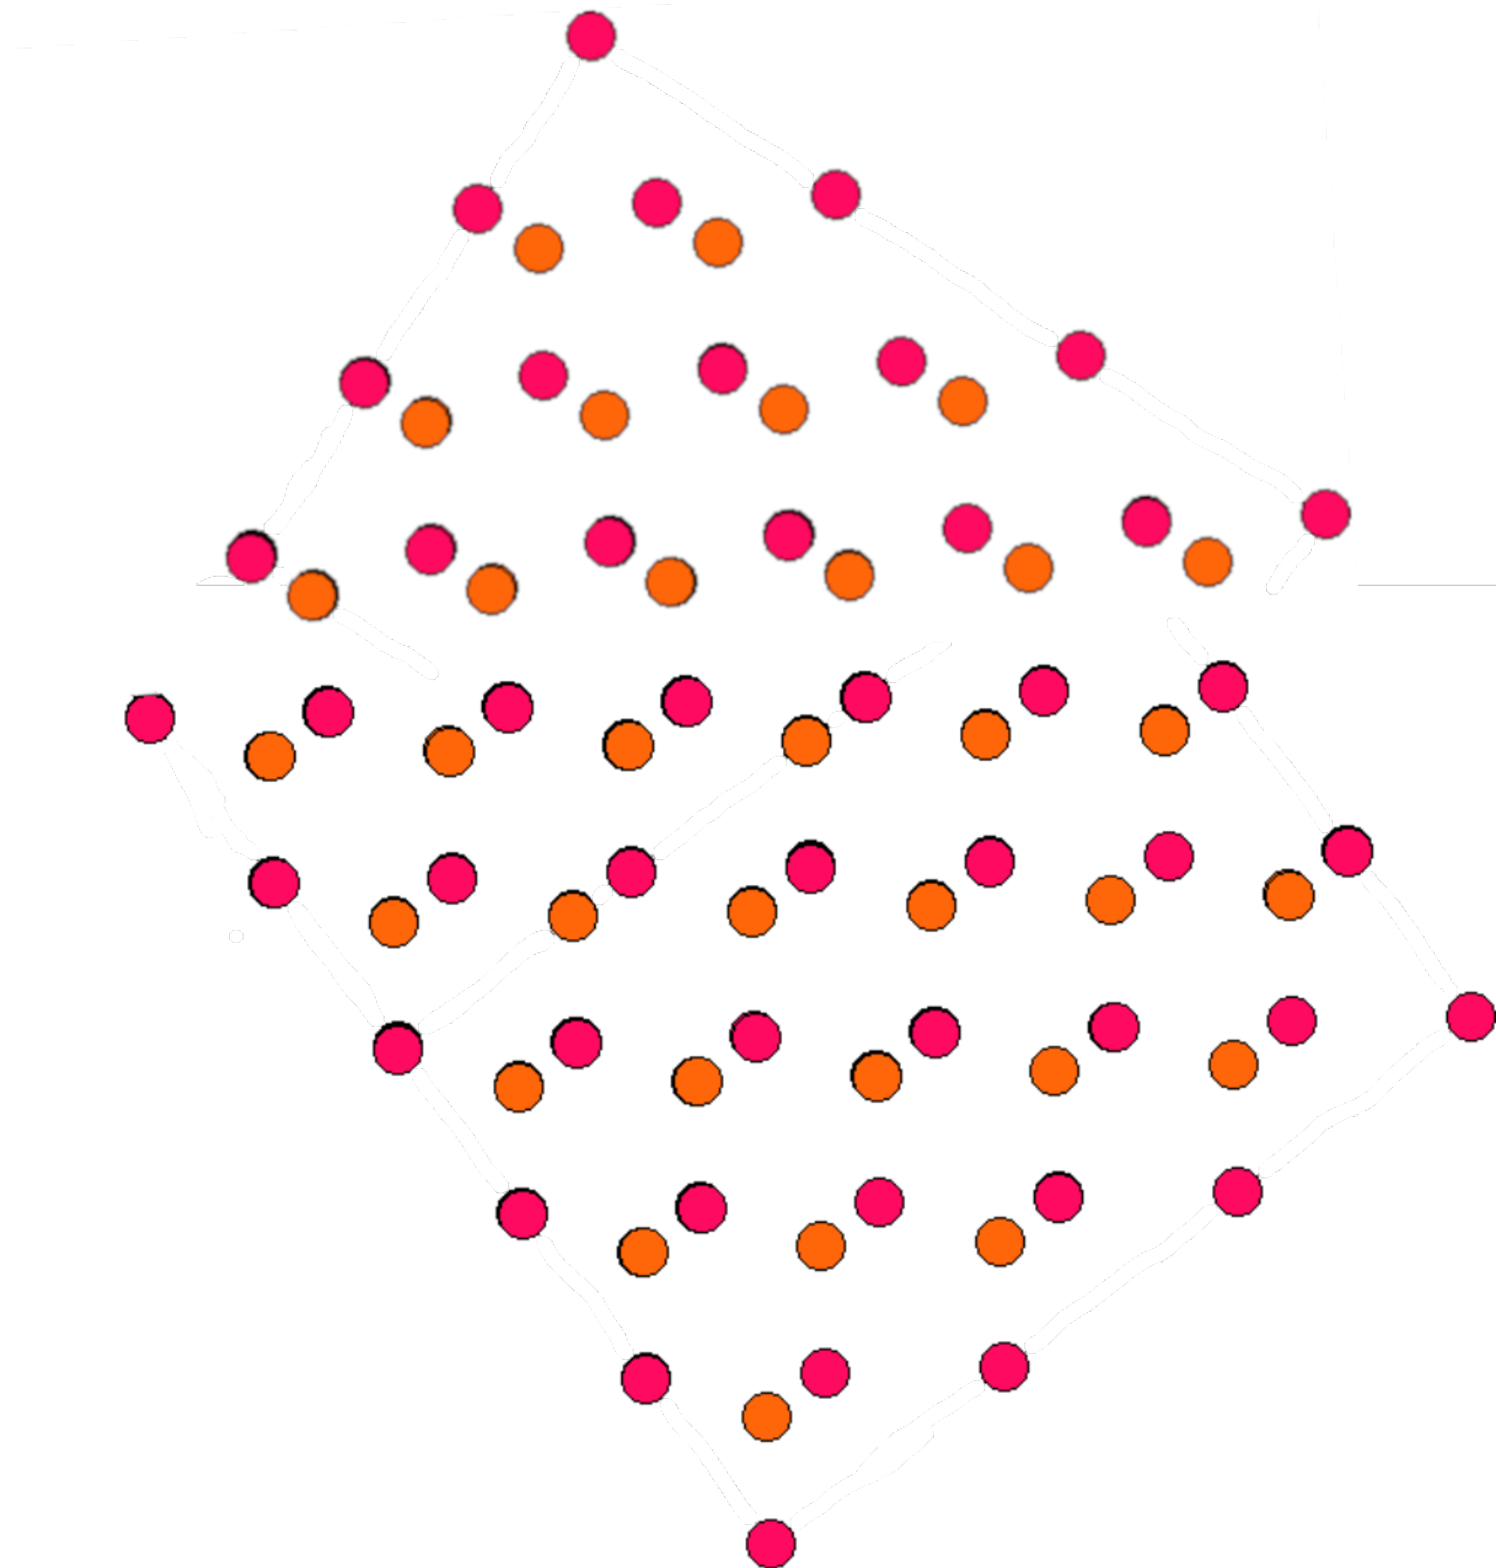
\includegraphics[width=0.3\textwidth]{2_Literature_Review/Fig/GaAs_rtp.pdf}};
        \draw [dashed] (-2.5,0.4) -- ++ (5,0.15) node [anchor = west] {RTP};
    \end{tikzpicture}
    \caption[Drawing of a \hkl{1 1 1} \acl{rtp} in a F\(\bar{4}\)3m crystal.]{Drawing of a \acl{rtp}, highlighted by a dashed line, corresponding to a \hkl{1 1 1} plane in a \acs{gaas} F\(\bar{4}\)3m crystal.}
    \label{fig:GaAs_rtp}
\end{figure}

Figure~\ref{fig:GaAs_rtp} shows a drawing of a \acf{rtp} corresponding to a \hkl{1 1 1} plane in a \acs{gaas} F\(\bar{4}\)3m crystal. Formation of this type of 2D defect is common in the growth of III-V crystals \cite{Borg2017} and its quantity is very sensitive to changes in the growth environment \cite{Algra2008, Chi2013} due to its low formation energy. From a lattice symmetry point of view, the \acs{rtp} is formed by adding a two-fold rotation axis to the \hkl{1 1 1} direction of the crystal. The two atomic bilayers adjacent to the \acs{rtp} can be considered a thin slice of wurtzite \cite{Glas2007, Vedel2022}.

Both atomic species and lattice symmetry affect the electronic properties of crystals. Bloch functions are the eigenfunctions of the Hamiltonian that describe a particle in a periodic potential \cite{Dirl2005}, and pose the basis for understanding the behaviour of electrons in crystals. They are also periodic functions, and in reciprocal space they are used to describe the electronic band structure, resulting in plots such as those in Figure~\ref{fig:band_structure}. The band structures in this figure were calculated, using \acf{dft}, and then plotted by Christian Dam Vedel. Energy is on the vertical axis, with its origin at the Fermi energy, which is the energetic midpoint between the last occupied state and the first unoccupied state, at \qty{0}{\kelvin} (thermal zero). The horizontal axis shows wavevectors along certain high-symmetry directions in the unit cell of the reciprocal lattice: the Brillouin zone \cite{Setyawan2010}. The energy of each of the states along the one-dimensional paths that link these points is then plotted. Therefore, in Figure~\ref{fig:band_structure}, the states below the Fermi energy are part of the valence band and those above it are part of the conduction band. 

\begin{figure}
    \centering
    \subcaptionbox{
        Band structure of F\(\bar{4}\)3m \acs{inp}.
        \label{subfig:ZB_bands_InP}
    }{
        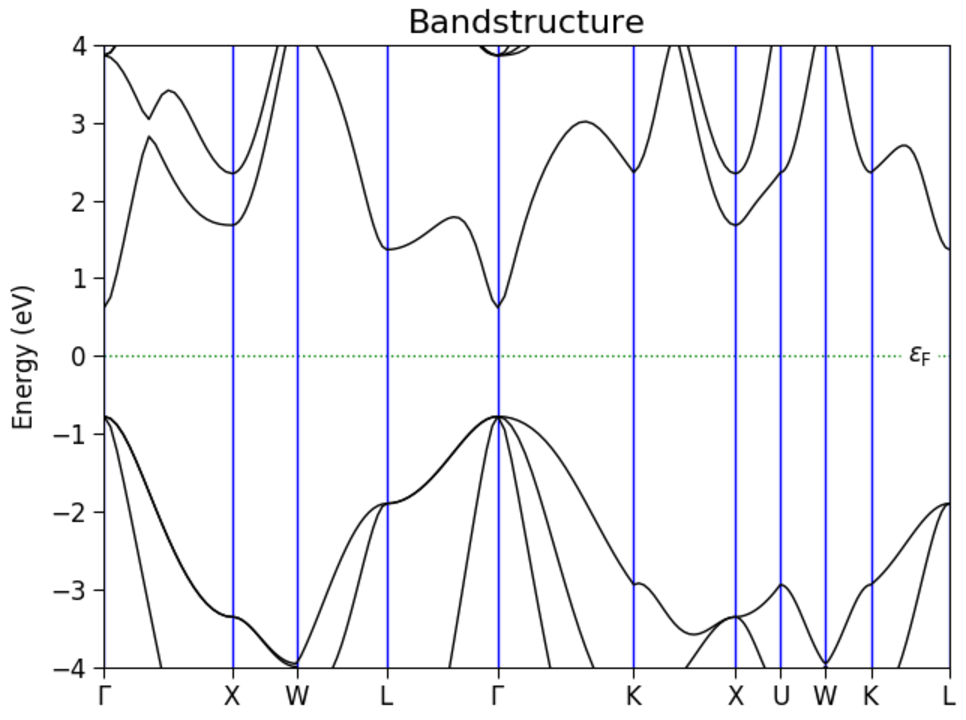
\includegraphics[width=0.48\textwidth]{2_Literature_Review/Fig/Zincblende_bandstructure_InP.pdf}
    }
    \subcaptionbox{
        Band structure of P6\(_3\)mc \acs{inp}.
        \label{subfig:WZ_bands_InP}
    }{
        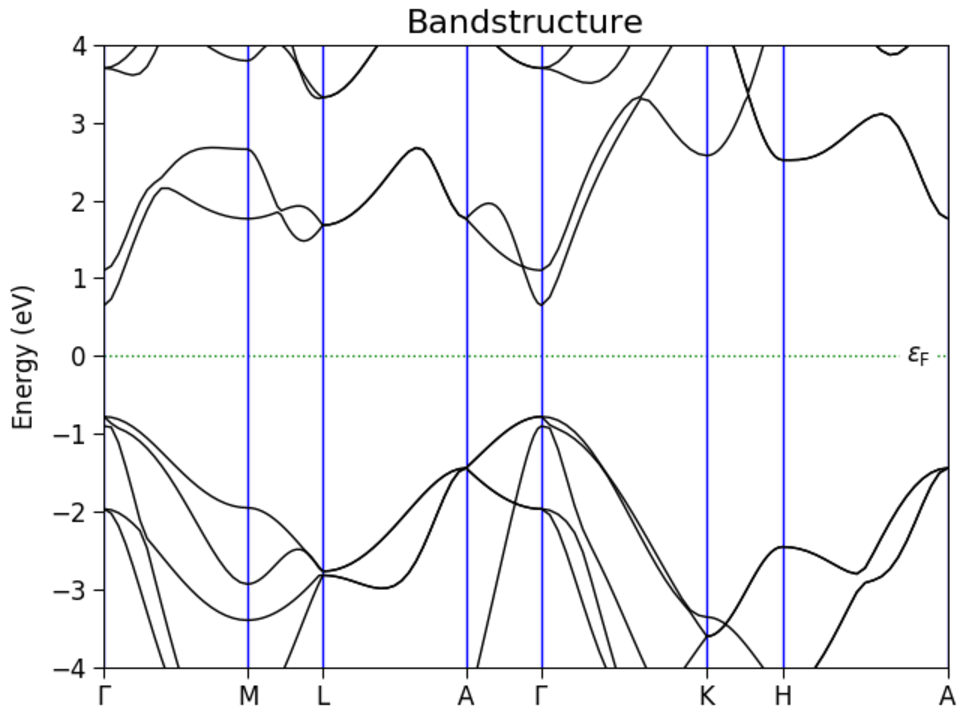
\includegraphics[width=0.48\textwidth]{2_Literature_Review/Fig/Wurtzite_bandstructure_InP.pdf}
    }
    \subcaptionbox{
        Band structure of Fd\(\bar{3}\)m \acs{si}.
        \label{subfig:Si_bands}
    }{
        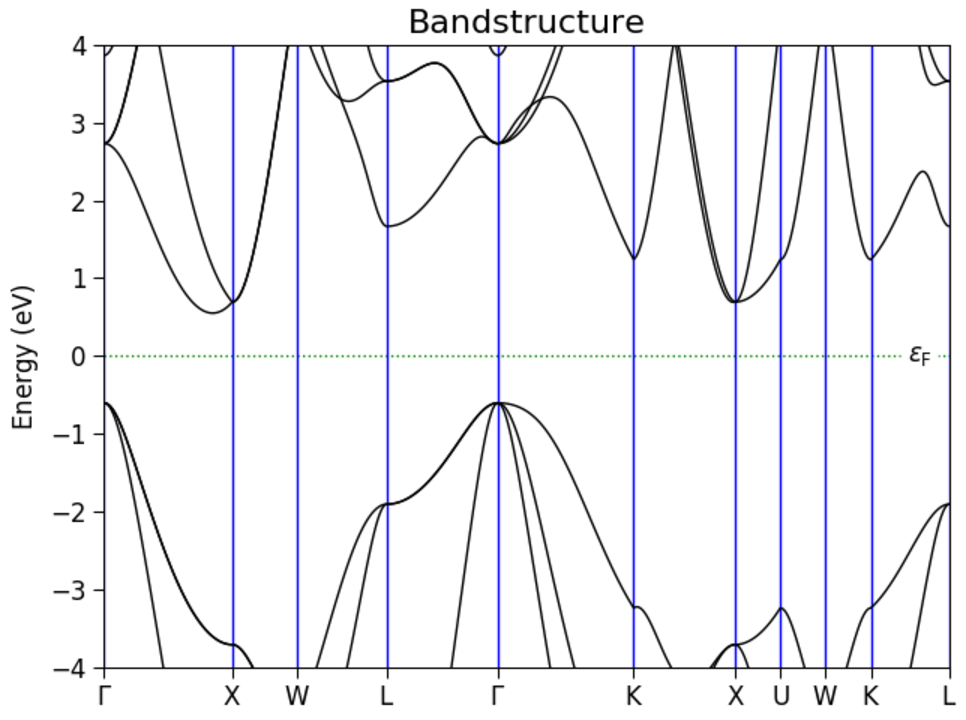
\includegraphics[width=0.48\textwidth]{2_Literature_Review/Fig/Silicon_bandstructure.pdf}
    }
    \caption[Band structures of \acl{si}, and \acs{inp} in its cubic and hexagonal phases.]{Band structures of \acl{si}, and \acs{inp} in its cubic and hexagonal phases, calculated with \acs{dft}. \subref{subfig:ZB_bands_InP} and \subref{subfig:WZ_bands_InP} show the band structures of zincblende and wurtzite \acs{inp}. \subref{subfig:Si_bands} shows the band structure of Fd\(\bar{3}\)m \acs{si}. Images courtesy of Christian Dam Vedel.}
    \label{fig:band_structure}
\end{figure}

The $\Gamma$ point is the centre of the Brillouin zone and is very important for understanding photon-driven electronic transitions between bands. Indeed, due to momentum conservation rules, a single photon can only cause what are called centrezone transitions, which are transitions between states at the $\Gamma$ point. Interband transitions outside of the centrezone require a third particle, usually a phonon, to mediate the transition, changing the type of interaction from two-particle to three-particle; which has a lower probability of occurring. This means that if the minimum of the conduction band and the maximum of the valence band are at the $\Gamma$ point, a material has a better chance to promote an electron when it is hit by a photon at the band gap energy. A material with this type of band structure is said to have a direct band gap. Conversely, a material that has a band structure with the minimum of the conduction band at a wavevector that is different from the wavevector of the maximum of the valence band is said to have an indirect band gap. Similarly, the radiative relaxation pathway is prevalent in direct band-gap semiconductors and non-radiative relaxation paths are prevalent in indirect band-gap semiconductors, affecting the light-emitting properties of these materials.

III-V semiconductors have direct band gaps, as exemplified by those of the zincblende and wurtzite phases of  \acl{inp} shown in Figures~\ref{subfig:ZB_bands_InP} and \ref{subfig:WZ_bands_InP}. This property is key in making III-Vs highly efficient light emitters and absorbers. On the contrary, \acl{si} has an indirect bandgap, as shown in Figure~\ref{subfig:Si_bands}, making it an ill-suited material for light emission and absorption.

It follows that tuning the band-gap of the material is very important for controlling the absorption and emission wavelengths. Although binary III-Vs provide fixed starting points in both band-gap and lattice constant, ternary and quaternary III-V compounds allow high-precision tuning of both properties \cite{Ning2017}. For example, the materials chosen by the \acs{design} consortium were \acs{inp} and \ce{In0_.53Ga)_.47As}, precisely because they are lattice-matched and therefore a lower density of defects is expected at their interface \cite{Pearsall1980, Sugii1983, Wagner1970}.

\section{\texorpdfstring{III-V-on-\acs{si} integration routes}{III-V-on-Si integration routes}}
Various III-V synthesis methods are available \cite{Kuech2016}: the following is an overview of epitaxial growth methods focussing on the integration routes of III-V semiconductors on \acl{si}, which can be divided into two broad categories: transfer and monolithic integration.

\subsection{Transfer integration}
Transfer integration refers to the indirect integration of III-V material grown on a different lattice-matched substrate on a \acl{si} wafer. 

The main advantage of these techniques is the absence of lattice mismatch as a source of defects during epitaxial growth. Furthermore, it allows the selection of the best-performing structures to be transferred onto the \acl{si} substrate \cite{Zadeh2016, Wang2017}. Transfer integration does not have to compromise on the growth parameters or material systems to achieve \acs{cmos} compatibility (except for bonding temperature). Together, the various methods that fall under this definition form a mature technology well established in industry \cite{Han2022, Wang2017}, and, as a result, benefit from years of industrial optimisation.

This type of integration requires the growth of III-V in a separate fabrication line that must maintain the high precision and cleanliness standard of the main \acs{cmos} \acl{si} line, resulting in a large capital investment. Furthermore, most classic transfer steps can result in a material with a more irregular geometry (wafer bow, surface roughness after etching), or presenting transfer-related defects \cite{Jevtics2022}, or require an extra bonding layer \cite{Tang2019, Jevtics2022}, and do not allow nanometre precision in integration \cite{McPhillimy2020, Wang2017}. However, the most advanced techniques that bypass most of these quality issues are too slow to provide a competitive transfer time for large, densely integrated \qty{200}{\milli\metre} (or \qty{300}{\milli\metre}) production wafers \cite{McPhillimy2020, Wang2017}.

\subsection{Monolithic integration}

Monolithic integration refers to direct integration by epitaxial growth of III-V semiconductors on a \acl{si} substrate. 

It naturally provides advantages such as extremely high spatial precision and accuracy for small device integration on wafer-scale substrates, which can be achieved in a shorter time frame compared to its heterogeneous analogues \cite{Wang2017}. It has the potential to be a more economical alternative to heterogeneous integration. If the growth process can be integrated with current \acs{cmos} processes, its implementation in a \acs{cmos} line would eliminate the need to have a dedicated III-V fabrication facility running in parallel with a \acl{si}-based plant unnecessary, especially if the use of III-V electronics is envisioned at the same time as III-V photonics \cite{Wang2017}. Thus, monolithic integration has the potential to reduce the capital cost required to integrate III-V photonics in different \acl{si}-based devices \cite{Tang2019}.

The main disadvantage of monolithic integration is the high lattice mismatch between \acl{si} and most III-V materials \cite{Kuech2016}. The effect of this mismatch in the material is the formation of strain-relaxing defects at the \acl{si} / III-V heterointerface \cite{Kunert2018, Shi2021}: these defects have a very detrimental effect on the performance and lifetime of a device \cite{Mahajan2000, Zenari2021}, and act as scattering or recombination centres \cite{Jeon2015}. The polar nature of III-V atomic bonds compared to nonpolar \acs{si}-\acs{si} bonds means that anti-phase boundaries can be created during growth on \acl{si} surfaces with monoatomic steps \cite{Kunert2018}, and most known surface treatments to eliminate nucleation sites for these defects occur in temperature ranges that are incompatible with the \acs{cmos} process \cite{Miller2000}. Furthermore, materials that are known to grow at a higher temperature, such as III – nitrides, and others that could have detrimental effects on the passivating of \acf{sio2} layers, such as gallium \cite{Miller2000}, also pose the same temperature-related \acs{cmos} compatibility issues. Another key obstacle, especially related to the direct growth of micro- and nanostructures, is the stricter requirements for the reproducibility and reliability of the process.

There are many monolithic integration routes and the most common categories are introduced in the following paragraphs.

\paragraph{Planar growth} Direct planar growth of III-Vs on \acl{si} is the simplest method of monolithic integration. It can be suitable for the growth of III-Vs with a lattice constant very close to that of \acl{si} or for the self-assembled nucleation of nanoparticles in a Stranski-Krastanov growth mode, which can pose the basis for quantum dot fabrication \cite{Shi2016, Reithmaier2016}. It, however, presents a few drawbacks related to the absence of a way to contain defects and the different material properties of the material stack \cite{Ravash2012}. It can lead to wafer bow or warp due to the mismatch of thermal coefficients between the various materials \cite{Miyoshi2016, Wang2017_2}, and materials with a high deviation from the \acl{si} lattice parameter can require strain management layers of \qty{1}{\micro\metre} or more to grow without defects \cite{Wang2017_2, Cantoro2012, Huang2022}.
\par
\paragraph{\Acf{sag}} \acs{sag} consists in the growth of III-V material from \acl{si} seeds located in openings in a horizontal mask of a material that does not promote nucleation, such as \acs{sio2}. These holes can be defined with different methods, from self-assembled masking to lithography. This type of growth results in nanostructures \cite{Cantoro2012} such as nanowires, both of a single material and in core-shell configurations with very high position control \cite{Tomioka2011}. Wafer bow and warp are not issues with \acs{sag}, since growth does not, unless promoted by accentuating lateral growth \cite{McKenzie2023}, end up forming a single material layer. However, in this technique, growth develops mainly in the vertical direction, and the presence of lateral growth can result in unwanted heterointerfaces.
\par
\paragraph{Droplet epitaxy} Droplet or \acf{vls} epitaxy consists in guiding the nucleation of III-V material by using a nano-droplet of a catalyst metal on the \acl{si} substrate. This technique also avoids wafer bow as it only results in the growth of nanowires \cite{Wagner1964}. Since \acs{vls} is dependent on the metallic droplet, the growth can be tuned to achieve high directionality and the incorporation of heterostructures with minimal or no unwanted side growth \cite{Harmand2018, Joyce2007}. This type of growth depends on the metal droplets and therefore on their self-assembled distribution on the substrate surface, which diminishes position control \cite{Joyce2007}. Similarly, the geometry of the resulting structures is limited to nanowires \cite{Wagner1964}, and the reservoir effect in the catalyst droplet complicates the control of composition in ternary and quaternary III-V materials \cite{Dubrovskii2017}. Nonetheless, this method allows for sophisticated growth studies such as in-situ TEM imaging \cite{Maliakkal2020, Jacobsson2016, Harmand2018}, leading to the possible refinement of growth recipes to the point where phase control can be achieved \cite{Algra2008, Caroff2009, Joyce2007}.
\par
\paragraph{\Acf{art}} \acs{art} refers to the confinement of defects to the seed region by sidewalls and other such barriers in a growth regimen mediated by a template. The basic idea is that, as most defects nucleate near the \acl{si} / III-V interface and then propagate in directions that are often not parallel to the growth axis, they can be trapped in the region of the material closest to the seed by sidewalls that constrict the III-V crystal so that it grows in a cavity with a high aspect ratio. 

\acs{sag}-\acs{art} has the mask selecting the seed areas increase in thickness to allow the trapping of defects. This technique also allows high position control of the III-V crystal, while accentuating control over the defects \cite{Han2016, Han2016_2}. However, typically \acs{sag}-\acs{art} employs large templates, which means that defects propagating in directions that lie in the plane of the side walls are not filtered by the \acs{art} mechanism \cite{Kunert2018}. Simultaneously, multiple nucleation points in large seed areas can result in grain boundaries that must be eliminated with additional process steps \cite{Kunert2016}.
\par
\paragraph{\Acf{tase}} \acs{tase} can be seen as an evolution of the \acs{sag}-\acs{art} method as it also defines \acl{si} seeds surrounded by \acs{sio2} and uses templates with high aspect ratio to guide the growth. The main difference with \acs{sag}-\acs{art} are the size and complexity of the templates and the focus on planar growth. \acs{tase} enables the growth of various vertical and horizontal nanostructures while maintaining extremely accurate geometry and position control \cite{Ritter2021, Tiwari2020, Schmid2015}. It also enables superior defect control, even compared with \acs{art}: far from the growth interface, defects can be effectively limited to twin planes \cite{Han2020}, which can also be eliminated in some cases \cite{Knoedler2017}. In certain geometries, it also enables phase control \cite{Staudinger2018}. 

On the other hand, it is the most complex method of those listed in terms of overall steps before III-V growth. Furthermore, since nanowires fill templates quickly, \acs{tase} can only grow core-shell structures in a microdisk format \cite{Tiwari2020} and not in nanowire format. 
\par

\section{\texorpdfstring{State of \acl{tase}}{State of template assisted selective epitaxy}}

As shown in the previous section, \acs{tase} is one of the most advanced monolithic integration techniques; its implementation can be found in Appendix~\ref{chap:tase}. The flexibility of \acs{tase} is demonstrated by the different ways research groups have used it. A group at the University of California Santa Barbara used \acs{tase} to achieve high facet control in the homoepitaxial growth of III-V semiconductors \cite{Brunelli2019, Goswami2020, Goswami2021}, while another group at the University of Hong Kong focussed on deposition in large templates \cite{Han2020, Yan2021} to then etch them into the desired device shape \cite{Han2020_2, Huang2024}. Sometimes the name \acf{lart} is used to highlight the use of large templates to create in-plane structures inside templates \cite{Han2020_2}. This method increases the risk of multiple nucleations and limits the defect-trapping effect in the in-plane direction \cite{Han2020, Yan2021, Huang2024}. 

The Hong Kong and IBM Research Europe Zurich groups have been developing template-based methods to fully integrate \acs{pic} on a \acs{soi} platform. This means a circuit complete of emitters, waveguides, and detrectors. With the \acs{tase} method, \acl{si} waveguides can be defined in the same lithography step as the emitting and absorbing structures, allowing for high design accuracy. Emitters can be integrated in the form of microdisks \cite{Tiwari2020, Tiwari2021} or modulators \cite{Scherrer2022, Scherrer2024}

















111B growth outside of tase

\section{Characterization of nano- and microstructures}

TALK ABOUT IMPORTANCE OF SINGLE FACET FOR INCORPORATION RATES (SEE FOLLOWING SECTION)

\section{Article 2}

Due to the presence of the SiO2 template, the quantum wells
develop only axially and not laterally. This results in improved
composition control in heterolayers of ternary III-V
compounds incorporated in the nanowires\cite{Borg2019} and therefore is
expected to allow for better control of the emission spectra.